\subsection*{Постановка задачи}
Основывываясь на вышеизложенном, была предложена следующая формулировка задачи, решение которой предполагается выполнять:

<<Пусть имеется $n$ требований к ПО, которые трассируются на $m$ файлов исходного кода. Файлы распределены по $k$ плагинам. Требуется определить оптимальное распределение файлов по плагинам для минимальной стоимости сопровождения возможных поставок в заявленных $l$ комплектациях. Стоимость сопровождения требования в рамках поставки зависит от состава поставки и может изменяться от наличия или отсутствия реализованных в поставке других требований>>.

\subsection*{Комплектации}
Решение, выполненное в виде комплекса плагинов, может быть поставлено более чем в одной комплектации. В рамках каждой из заявленных комплектаций каждое из возможных требований маркируется либо как \textit{полезное}, либо как \textit{бесполезное}. Поставка должна включать все \textit{полезные} требования. Присвоенные признаки полезности каждому из требований во всех заявленных комплектациях образуют матрицу бинарных отношений $E_{l \times n}$. Элемент $e_{i, j} = 0$ если в рамках $i$-й комплектации $j$-е требование \textit{бесполезно} и $1$ если \textit{полезно}.

\subsection*{Цена постпродажного обслуживания}
Цена постпродажного обслуживания каждого отдельного требования может отличаться в разных поставках. Это происходит из-за того, что по условию задачи наличие других реализованных требований в поставке изменяет цену сопровождения требования и может его как уменьшать, так и увеличивать. Образуется матрица изменения стоимости сопровождения требований $C_{n \times n}$. В ней указывается, на сколько изменится цена сопровождения $i$-го требования, если в поставке будет реализовано $j$-е.

\subsection*{Трассируемость требований к ПО на файлы исходного кода}
Каждое требование трассируется на файлы исходного кода. Для реализации требования в поставке в нее должны быть включены все файлы, которые реализуют данное требование. При этом каждое из требований может быть реализовано в одном или нескольких файлах, а каждый файл может реализовывать одно или несколько требований. Так образуется матрица трассируемости $T_{n \times m}$. Каждый из элементов матрицы имеет значение в диапазоне $[0;1]$. Значение определяет условную долю участия файла в реализации требования. Если $j$-й файл не задействован в реализации $i$-го требования, то значение $t_{i, j} = 0$, иначе $0 < t_{i, j} \le 1$. При этом выполняются условия:
\begin{center}
  $\displaystyle \sum^{m}_{j = 1}t_{1, j} = 1, 
    \sum^{m}_{j = 1}t_{2, j} = 1, \cdots, \sum^{m}_{j = 1}t_{n, j} = 1$
\end{center}

\subsection*{Зависимости между файлами исходного кода}
Файлы исходного кода могут иметь зависимости друг на друга. Без разрешения зависимостей файл не может быть включен в поставку. Т.к. число возможных зависимостей у каждого из файлов не может превышать общее число файлов, зависимости между ними описывает матрица бинарных отношений $D_{m \times m}$. В ней элемент $d_{i, j} = 0$ если у $i$-го файла нет зависимости от $j$-го и равен $1$ если зависимость есть. Файл не зависит сам от себя. Поэтому значения элементов на главной диагонале равны $0$.

\subsection*{Распределение файлов исходного кода по плагинам}
Файлы исходного кода распределены по плагинам. Один файл может быть включен только в один плагин, в то время как один плагин может включать в себя множество файлов. Образуется матрица бинарных отношений $A_{m \times k}$. Элемент $a_{i, j} = 0$ если $i$-й файл не включен в $j$-й плагин и равен $1$ если включен. Кроме того на элементы матрицы $A$ действуют ограничения:
\begin{center}
  $\displaystyle \sum^{k}_{j = 1}a_{1, j} = 1, \sum^{k}_{j = 1}a_{2, j} = 1, \cdots, \sum^{k}_{j = 1}a_{m, j} = 1$
\end{center}
Решение задачи поиска оптимальной декомпозиции заключается в нахождении именно этих коэффициентов.

\subsection*{Целевая функция}
Целевая функция может быть записана как минимизация стоимостей поставок во всех возможных комплектациях:
\begin{center}
  $\displaystyle min \sum^{l}_{i = 1} f_{c}(E_{i})$
\end{center}

где $f_{c}$ - функция стоимости сопровождения комплектации. Алгоритм работы этой функции:

\begin{enumerate}
  \item Определить вектор полезных требований $R_{1 \times n}$. Является входным аргументом функции $f_{c}$.
  \item Вычислить вектор полезных файлов исходного кода:
  \begin{center}
    $F_{1 \times m} = R \cdot T$
  \end{center}
  \item Определить минимально необходимый перечень файлов исходного кода для осуществления поставки в заданной комплектации. Для этого вычислить сумму $F$ и разрешенных зависимостей: 
  \begin{center}
    $\displaystyle \hat{F}_{1 \times m} = F + \sum^{m}_{j = 1}f_{dep}(j)$
  \end{center}
  Описание функции $f_{dep}$ приведено далее.
  \item Определить плагины, которые должны войти в поставку:
  \begin{center}
    $P_{1 \times k} = f_{in}(\hat{F} \cdot A)$
  \end{center}
  \begin{center}
    $\dot{P}_{k \times 1} = P^{T}$
  \end{center}
  \begin{center}
    $
    f_{in} =
    \begin{cases}
      0 & \quad \text{если } x = 0 \\
      1 & \quad \text{если } x > 0
    \end{cases}
    $
  \end{center}
  \item Определить все файлы исходного кода, которые должны войти в поставку:
  \begin{center}
    $\dot{F}_{m \times 1} = A \cdot \dot{P}$
  \end{center}
  \item Определить все реализованные требования в поставке:
  \begin{center}
    $\dot{R}_{n \times 1} = f_{im}(T \cdot \dot{F})$
  \end{center}
  \begin{center}
    $
    f_{im} =
    \begin{cases}
      0 & \quad \text{если } x < 1 \\
      1 & \quad \text{если } x \geq 1
    \end{cases}
    $
  \end{center}
  \item Рассчитать стоимость сопровождения комплектации:
  \begin{center}
    $\dot{R}^{T} \cdot (C \cdot \dot{R})$
  \end{center}
\end{enumerate}

Таким образом целевая функция - это:
  \begin{center}
    $\displaystyle min \sum^{l}_{i = 1} \Bigg[\Bigg[f_{im}\Bigg(T \cdot \bigg(A \cdot \bigg[f_{in}\Big(\big(E_{i} \cdot T + \sum^{m}_{j = 1}f_{dep}(j)\big) \cdot A\Big)\bigg]^{T}\bigg)\Bigg)\Bigg]^{T} \cdot \Bigg[C \cdot~f_{im}\Bigg(T~\cdot~\bigg(A \cdot \bigg[f_{in}\Big(\big(E_{i} \cdot T + \sum^{m}_{j = 1}f_{dep}(j)\big) \cdot A\Big)\bigg]^{T}\bigg)\Bigg)\Bigg]\Bigg]$
  \end{center}

\subsection*{Функция разрешения зависимостей между файлами исходного кода}
Функция разрешения зависимостей между файлами исходного кода $f_{dep}$ позволяет определять перечень зависимостей среди файлов на каждом из слоев зависимостей. Слой зависимости определяет глубину, на которой проводится поиск зависимостей. Так, зависимости $F$ имеют уровень $1$. Их зависимости уровень $2$ и т.д. Заметим, что число слоев не может превышать общее число файлов исходного кода $m$.

Например, пусть задача решается для четырех файлов исходного кода. Ниже приведен пример вектора $F$ и матрицы $D$ для этого случая:
\begin{center}
  $
    F = \begin{pmatrix}
      1 & 0 & 0 & 0 
    \end{pmatrix}
  $
\end{center}
\begin{center}
  $
    D = \begin{pmatrix}
    0 & 1 & 0 & 0 \\
    0 & 0 & 1 & 1 \\
    0 & 0 & 0 & 0 \\
    0 & 0 & 0 & 0 
    \end{pmatrix}
  $
\end{center}
Значения элементов вектора $F$ говорят о том, что полезным является только первое требование. Значения элементов матрицы $D$ говорят, что:
\begin{itemize}
  \item Файл № $1$ имеет зависимость на файл № $2$
  \item Файл № $2$ имеет зависимости на файлы № $3$ и № $4$
  \item Файл № $3$ не имеет зависимостей
  \item Файл № $4$ не имеет зависимостей
\end{itemize}
Тогда зависимости уровня $1$:
\begin{center}
  $
  \begin{pmatrix}
    1 & 0 & 0 & 0 
  \end{pmatrix}
  \cdot
  \begin{pmatrix}
    0 & 1 & 0 & 0 \\
    0 & 0 & 1 & 1 \\
    0 & 0 & 0 & 0 \\
    0 & 0 & 0 & 0 
  \end{pmatrix}
  = 
  \begin{pmatrix}
    0 & 1 & 0 & 0 
  \end{pmatrix}
  $
\end{center}
У полезных файлов $F$ присутствует зависимость только на файл № $2$. Это соответствует заданной матрице $D$. Если полученный вектор умножить заново на матрицу $D$, то будут вычислены файлы для разрешения зависимостей их уровня:
\begin{center}
  $
  \begin{pmatrix}
    0 & 1 & 0 & 0 
  \end{pmatrix}
  \cdot
  \begin{pmatrix}
  0 & 1 & 0 & 0 \\
  0 & 0 & 1 & 1 \\
  0 & 0 & 0 & 0 \\
  0 & 0 & 0 & 0 
  \end{pmatrix}
  = 
  \begin{pmatrix}
    0 & 0 & 1 & 1 
  \end{pmatrix}
  $
\end{center}

Исходя из этого $f_{dep}$ можно записать как рекурсивную функцию:
\begin{center}
  $
  f_{dep}(x) = 
  \begin{cases}
    F \cdot D & \quad \text{если } x = 1 \\
    f_{dep}(x - 1) \cdot D & \quad \text{если } x > 1
  \end{cases}
  $
\end{center}
где $x$ - уровень вложенности зависимостей.

Примечателен тот факт, что значение элемента не важно. Если оно больше $0$, значит элемент активен.

\subsection*{Умножение бинарных параметров}
Функция перемножения бинарных параметров используется как альтернатива обычному перемножению для исключения в моделе нелинейности. Перемножение параметров приводит к появлению в моделе нелинейности. Наличие нелинейности в моделе приведет к значительному усложенению ее решения и невозможности ее решения большинством программных решателей.

С целью нивелирования этого обстоятельства целевая функция в частности и модель в целом должны быть переработаны. Переработка базируется на том обстоятельстве, что перемножаются не параметры в общем виде, а именно бинарные параметры. Произведение элементов $x \cdot y$, где $x$ и $y$ значения бинарных параметров, может быть заменено дополнительным бинарным параметром $f$, значение которого должно удовлетворять следующим ограничениям:
\begin{center}
  $
  \begin{cases}
    x + y <= f + 1 & \quad \text{в таблице \ref{tab:fbm} имеет обозначение } f_{1} \\
    f <= x     & \quad \text{в таблице \ref{tab:fbm} имеет обозначение } f_{2} \\
    f <= y     & \quad \text{в таблице \ref{tab:fbm} имеет обозначение } f_{3}
  \end{cases}
  $
\end{center}
Демонстрация робастности ограничений приведена в таблице \ref{tab:fbm}:
\begin{longtable}{|c|c|c|c|c|c|c|}
  \caption{Робастность ограничений $f_{bm}$}
  \label{tab:fbm}\\   
  \hline
  \cellcolor{gray} $x$ & 
  \cellcolor{gray} $y$ & 
  \cellcolor{gray} $f$ & 
  \cellcolor{gray} $f_{1}$ & 
  \cellcolor{gray} $f_{2}$ & 
  \cellcolor{gray} $f_{3}$ & 
  \cellcolor{gray} $f_{1} \vee f_{2} \vee f_{3}$ \\
  \endfirsthead
  \hline
  \cellcolor{gray} $x$ & 
  \cellcolor{gray} $y$ & 
  \cellcolor{gray} $f$ & 
  \cellcolor{gray} $f_{1}$ & 
  \cellcolor{gray} $f_{2}$ & 
  \cellcolor{gray} $f_{3}$ & 
  \cellcolor{gray} $f_{1} \vee f_{2} \vee f_{3}$ \\
  \endhead
  \endfoot
  \hline
  0 & 0 & 0 & true  & true  & true  & true \\
  \hline
  0 & 0 & 1 & true  & false & false & false \\
  \hline
  0 & 1 & 0 & true  & true  & true  & true \\
  \hline
  0 & 1 & 1 & true  & false & true  & false \\
  \hline
  1 & 0 & 0 & true  & true  & true  & true \\
  \hline
  1 & 0 & 1 & true  & true  & false & false \\
  \hline
  1 & 1 & 0 & false & true  & true  & false \\
  \hline
  1 & 1 & 1 & true  & true  & true  & true \\
  \hline
\end{longtable}

\subsection*{Функция определения вхождения}
Функция определения вхождения $f_{in}$ применяется с целью преобразования большего или равного $0$ входного параметра в бинарное значение.

Функцию $f_{in}$ следует представить в виде параметров и ограничений в модели. Для этого используется метод big M [\ref{lit:7}]. Этот метод предписывает заведение в моделе дополнительнго бинарного параметра $f$, значение которой должно удовлетворять следующим ограничениям:
\begin{center}
  $
  \begin{cases}
    f < x + 1 & \quad \text{в таблице \ref{tab:fin} имеет обозначение } f_{1} \\
    x \le M \cdot f & \quad \text{в таблице \ref{tab:fin} имеет обозначение } f_{2}
  \end{cases}
  $
\end{center}

Здесь $M$ - условно большое число. Демонстрация робастности ограничений приведена в таблице \ref{tab:fin}:
\begin{longtable}{|c|c|c|c|c|}
  \caption{Робастность ограничений $f_{in}$}
  \label{tab:fin}\\   
  \hline
  \cellcolor{gray} $x$ & 
  \cellcolor{gray} $f$ & 
  \cellcolor{gray} $f_{1}$ & 
  \cellcolor{gray} $f_{2}$ & 
  \cellcolor{gray} $f_{1} \vee f_{2}$ \\
  \endfirsthead
  \hline
  \cellcolor{gray} $x$ & 
  \cellcolor{gray} $f$ & 
  \cellcolor{gray} $f_{1}$ & 
  \cellcolor{gray} $f_{2}$ & 
  \cellcolor{gray} $f_{1} \vee f_{2}$ \\
  \endhead
  \endfoot
  \hline
  0              & 0 & true  & true  & true \\
  \hline
  0              & 1 & false & true  & false \\
  \hline
  (0 ; 1)        & 0 & true  & false & false \\
  \hline
  (0 ; 1)        & 1 & true  & true  & true \\
  \hline
  1              & 0 & true  & false & false \\
  \hline
  1              & 1 & true  & true  & true \\
  \hline
  (1 ; $\infty$) & 0 & true  & false & false \\
  \hline
  (1 ; $\infty$) & 1 & true  & true  & true \\
  \hline
\end{longtable}

\subsection*{Функция определения реализованности}
Функция определения реализованности $f_{im}$ применяется с целью преобразования большего или равного $0$ входного параметра в бинарное значение.

Функцию $f_{im}$ следует представить в виде параметров и ограничений в моделе. Для этого используется ранее упомянутый метод big M. Следуя ему, ограничения на значение дополнительного бинарного параметра $f$ следующие:
\begin{center}
  $
  \begin{cases}
    x \geq f & \quad \text{в таблице \ref{tab:fim} имеет обозначение } f_{1} \\
    x < M \cdot f + 1 & \quad \text{в таблице \ref{tab:fim} имеет обозначение } f_{2}
  \end{cases}
  $
\end{center}

Демонстрация робастности ограничений приведена в таблице \ref{tab:fim}:
\begin{longtable}{|c|c|c|c|c|}
  \caption{Робастность ограничений $f_{im}$}
  \label{tab:fim}\\   
  \hline
  \cellcolor{gray} $x$ & 
  \cellcolor{gray} $f$ & 
  \cellcolor{gray} $f_{1}$ & 
  \cellcolor{gray} $f_{2}$ & 
  \cellcolor{gray} $f_{1} \vee f_{2}$ \\
  \endfirsthead
  \hline
  \cellcolor{gray} $x$ & 
  \cellcolor{gray} $f$ & 
  \cellcolor{gray} $f_{1}$ & 
  \cellcolor{gray} $f_{2}$ & 
  \cellcolor{gray} $f_{1} \vee f_{2}$ \\
  \endhead
  \endfoot
  \hline
  0              & 0 & true  & true  & true \\
  \hline
  0              & 1 & false & true  & false \\
  \hline
  (0 ; 1)        & 0 & true  & true  & true \\
  \hline
  (0 ; 1)        & 1 & false & true  & false \\
  \hline
  1              & 0 & true  & false & false \\
  \hline
  1              & 1 & true  & true  & true \\
  \hline
  (1 ; $\infty$) & 0 & true  & false & false \\
  \hline
  (1 ; $\infty$) & 1 & true  & true  & true \\
  \hline
\end{longtable}

% Про ограничения и появление 1 / M
\subsection*{Описание строгих неравенств}
Часть ограничений модели описана при помощи знаков строгого неравенсва. Для будущей программной реализации необходимо задание ограничений на значения параметра при помощи только нестрогих неравенств. С целью нивелирования данного обстоятельства используется константа $1 / M$ - условно малое число. Тогда ограничение модели вида $x < y$ будет описано как $x + 1 / M \le y$.

\subsection*{Построение математической модели}
В качестве примера приводится математическая модель, размеры исходных матриц которых соответствуют следующим величинам:
\begin{center}
  $l = 1, n = 5, m = 4, k = 3$
\end{center}

В качестве входных значений используются следующие матрицы:
\begin{center}
  $
  T = 
  \begin{pmatrix}
      1 &   0 &   0 & 0   \\
    0.5 & 0.5 &   0 & 0   \\
      0 & 0.5 & 0.5 & 0   \\
      0 &   0 & 0.5 & 0.5 \\
      0 &   0 &   0 & 1 
  \end{pmatrix}
  $
\end{center}

\begin{center}
  $
  D = 
  \begin{pmatrix}
    0 & 0 & 1 & 0   \\
    0 & 0 & 1 & 1   \\
    0 & 0 & 0 & 0   \\
    0 & 0 & 0 & 0 
  \end{pmatrix}
  $
\end{center}

\begin{center}
  $
  C = 
  \begin{pmatrix}
    1 & 1 & 1 & 1 & 1   \\
    1 & 1 & 1 & 1 & 1   \\
    1 & 1 & 1 & 1 & 1   \\
    1 & 1 & 1 & 1 & 1   \\
    1 & 1 & 1 & 1 & 1 
  \end{pmatrix}
  $
\end{center}

\begin{center}
  $
  E = \begin{pmatrix}
    1 & 0 & 0 & 0 & 0
  \end{pmatrix}
  $
\end{center}

Представление в виде графа, построенного в соответствии с описанными выше исходными данными модели, изображено на рисунке \ref{fig:graph}.

\begin{figure}[H]
  \centering
  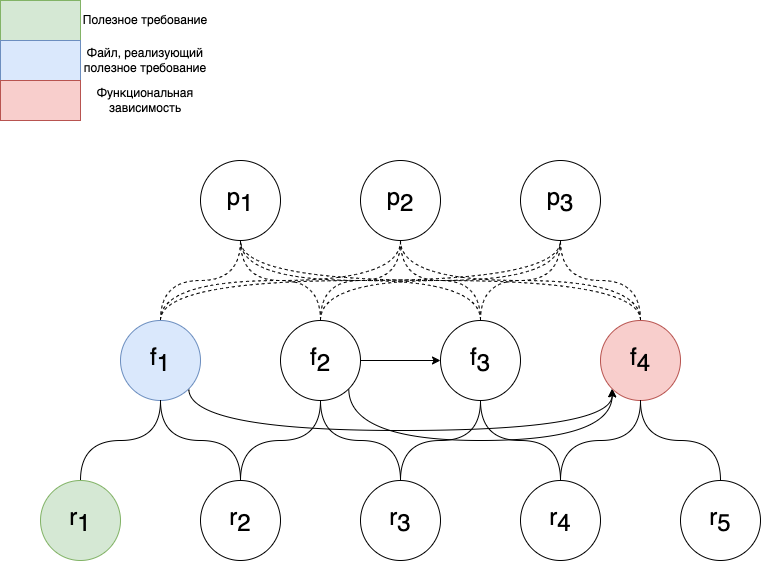
\includegraphics[width=1\textwidth]{graph}
  \caption{Предствление в виде графа}
  \label{fig:graph}
\end{figure}

Построение математической модели по шагам:
\begin{enumerate}
  \item Бинарные параметры матрицы $A$ дополняют модель следующими ограничениями:
  \begin{center}
    $
      \begin{cases}
        a_{1,1} + a_{1,2} + a_{1,3} = 1 \\ % 1
        a_{2,1} + a_{2,2} + a_{2,3} = 1 \\ % 2
        a_{3,1} + a_{3,2} + a_{3,3} = 1 \\ % 3
        a_{4,1} + a_{4,2} + a_{4,3} = 1 % 4
      \end{cases}
    $
  \end{center}
  \item Вектор полезных требований $R_{1 \times 5}$
  \begin{center}
    $
      R = 
      \begin{pmatrix}
        1 & 0 & 0 & 0 & 0
      \end{pmatrix}
    $
  \end{center}
  
  \item Вектор полезных файлов исходного кода $F_{1 \times 4}$
  \begin{center}
    $
      R \cdot T = 
      \begin{pmatrix}
        1 & 0 & 0 & 0 & 0
      \end{pmatrix}
      \cdot
      \begin{pmatrix}
        1 &   0 &   0 & 0   \\
      0.5 & 0.5 &   0 & 0   \\
        0 & 0.5 & 0.5 & 0   \\
        0 &   0 & 0.5 & 0.5 \\
        0 &   0 &   0 & 1 
    \end{pmatrix}
    = \begin{pmatrix}
        1 & 0 & 0 & 0
      \end{pmatrix}
    $
  \end{center}
  
  \item Разрешение зависимостей полезных файлов исходного кода $\displaystyle \sum^{m}_{j = 1}f_{dep}(j)$
  \begin{center}
    $
      f_{dep}(1) = 
      \begin{pmatrix}
        1 & 0 & 0 & 0
      \end{pmatrix}
      \cdot
      \begin{pmatrix}
        0 & 0 & 1 & 0   \\
        0 & 0 & 1 & 1   \\
        0 & 0 & 0 & 0   \\
        0 & 0 & 0 & 0 
      \end{pmatrix}
      = \begin{pmatrix}
          0 & 0 & 1 & 0
        \end{pmatrix}
    $
  \end{center}
  \begin{center}
    $
      f_{dep}(2) = 
      \begin{pmatrix}
        0 & 0 & 1 & 0
      \end{pmatrix}
      \cdot
      \begin{pmatrix}
        0 & 0 & 1 & 0   \\
        0 & 0 & 1 & 1   \\
        0 & 0 & 0 & 0   \\
        0 & 0 & 0 & 0 
      \end{pmatrix}
      = \begin{pmatrix}
          0 & 0 & 0 & 0
        \end{pmatrix}
    $
  \end{center}
  \begin{center}
    $
      f_{dep}(3) = 
      \begin{pmatrix}
        0 & 0 & 0 & 0
      \end{pmatrix}
      \cdot
      \begin{pmatrix}
        0 & 0 & 1 & 0   \\
        0 & 0 & 1 & 1   \\
        0 & 0 & 0 & 0   \\
        0 & 0 & 0 & 0 
      \end{pmatrix}
      = \begin{pmatrix}
          0 & 0 & 0 & 0
        \end{pmatrix}
    $
  \end{center}
  \begin{center}
    $
      f_{dep}(4) = 
      \begin{pmatrix}
        0 & 0 & 0 & 0
      \end{pmatrix}
      \cdot
      \begin{pmatrix}
        0 & 0 & 1 & 0   \\
        0 & 0 & 1 & 1   \\
        0 & 0 & 0 & 0   \\
        0 & 0 & 0 & 0 
      \end{pmatrix}
      = \begin{pmatrix}
          0 & 0 & 0 & 0
        \end{pmatrix}
    $
  \end{center}
  \begin{center}
    $
      f_{dep}(1) + f_{dep}(2) + f_{dep}(3) + f_{dep}(4) = 
      \begin{pmatrix}
          0 & 0 & 1 & 0
        \end{pmatrix}
      +
      \begin{pmatrix}
        0 & 0 & 0 & 0
      \end{pmatrix}
      +
      \begin{pmatrix}
        0 & 0 & 0 & 0
      \end{pmatrix}
      +
      \begin{pmatrix}
        0 & 0 & 0 & 0
      \end{pmatrix}
      =
      \begin{pmatrix}
        0 & 0 & 1 & 0
      \end{pmatrix}
    $
  \end{center}
  \item Полезные файлы исходного кода с разрешенными зависимостями $\hat{F}_{1 \times m}$
  \begin{center}
    $
      \displaystyle F + \sum^{m}_{j = 1}f_{dep}(j) = 
      \begin{pmatrix}
        1 & 0 & 0 & 0
      \end{pmatrix}
      +
      \begin{pmatrix}
        0 & 0 & 1 & 0
      \end{pmatrix}
      =
      \begin{pmatrix}
        1 & 0 & 1 & 0
      \end{pmatrix}
    $
  \end{center}
  \item Плагины, которые должны войти в поставку $P_{1 \times k}$ 
  \begin{center}
    $
      \hat{F} \cdot A 
      = 
      \begin{pmatrix}
        1 & 0 & 1 & 0
      \end{pmatrix}
      \cdot
      \begin{pmatrix}
        a_{1, 1} & a_{1, 2} & a_{1, 3} \\
        a_{2, 1} & a_{2, 2} & a_{2, 3} \\
        a_{3, 1} & a_{3, 2} & a_{3, 3} \\
        a_{4, 1} & a_{4, 2} & a_{4, 3}
      \end{pmatrix}
      =
      \begin{pmatrix}
        a_{1, 1} + a_{3, 1} & 
        a_{1, 2} + a_{3, 2} & 
        a_{1, 3} + a_{3, 3} 
      \end{pmatrix}
    $
  \end{center}
  Применяя функцию $f_{in}$ образуется вектор выражения в матрице заменяются дополнительными бинарными параметрами.
  
  $a_{1, 1} + a_{3, 1}$ заменяется на $f_{1}$ с добавлением в моделе следующих ограничений:
  \begin{center}
    $
      \begin{cases}
        -\infty \le f_{1} + 1 / M - (a_{1,1} + a_{3,1} + 1) \le 0 \\ % 5
        -\infty \le a_{1,1} + a_{3,1} - M \cdot f_{1} \le 0 % 6
      \end{cases}
    $
  \end{center}
  $a_{1, 2} + a_{3, 2}$ заменяется на $f_{2}$ с добавлением в моделе следующих ограничений:
  \begin{center}
    $
      \begin{cases}
        -\infty \le f_{2} + 1 / M - (a_{1,2} + a_{3,2} + 1) \le 0 \\ % 7
        -\infty \le a_{1,2} + a_{3,2} - M \cdot f_{2} \le 0 % 8
      \end{cases}
    $
  \end{center}
  $a_{1, 3} + a_{3, 3}$ заменяется на $f_{3}$ с добавлением в моделе следующих ограничений:
  \begin{center}
    $
      \begin{cases}
        -\infty \le f_{3} + 1 / M - (a_{1,3} + a_{3,3} + 1) \le 0 \\ % 9
        -\infty \le a_{1,3} + a_{3,3} + M \cdot f_{3} \le 0 % 10
      \end{cases}
    $
  \end{center}
  \begin{center}
    $
      \dot{P} = \begin{pmatrix}
        f_{1} \\ 
        f_{2} \\
        f_{3} 
      \end{pmatrix}
    $
  \end{center}
  \item Файлы исходного кода, которые должны войти в поставку $\dot{F}_{m \times 1}$
  \begin{center}
    $
    A \cdot \dot{P} =
    \begin{pmatrix}
      a_{1, 1} & a_{1, 2} & a_{1, 3} \\
      a_{2, 1} & a_{2, 2} & a_{2, 3} \\
      a_{3, 1} & a_{3, 2} & a_{3, 3} \\
      a_{4, 1} & a_{4, 2} & a_{4, 3}
    \end{pmatrix}
    \cdot
    \begin{pmatrix}
      f_{1} \\ 
      f_{2} \\
      f_{3} 
    \end{pmatrix}
    =
    \begin{pmatrix}
      a_{1, 1} \cdot f_{1} + a_{1, 2} \cdot f_{2} + a_{1, 3} \cdot f_{3} \\ 
      a_{2, 1} \cdot f_{1} + a_{2, 2} \cdot f_{2} + a_{2, 3} \cdot f_{3} \\
      a_{3, 1} \cdot f_{1} + a_{3, 2} \cdot f_{2} + a_{3, 3} \cdot f_{3} \\ 
      a_{4, 1} \cdot f_{1} + a_{4, 2} \cdot f_{2} + a_{4, 3} \cdot f_{3} 
    \end{pmatrix}
    $
  \end{center}
  Получившиеся выражения в элементах матрицы нелинейны. Однако в силу того, что элементы матрицы $A$ и параметры $f_{1}, f_{2}$ и $f_{3}$ бинарны, можно привести их к линейности посредством замены выражений дополнительными бинарными параметрами.
  
  $a_{1, 1} \cdot f_{1}$ заменяется на $f_{4}$ с добавлением в моделе следующих ограничений:
  \begin{center}
    $
      \begin{cases}
        -\infty \le f_{1} + a_{1,1} - (f_{4} + 1) \le 0 \\ % 11
        -\infty \le f_{4} - f_{1} \le 0 \\ % 12
        -\infty \le f_{4} - a_{1,1} \le 0 % 13
      \end{cases}
    $
  \end{center}
  $a_{1, 2} \cdot f_{2}$ заменяется на $f_{5}$ с добавлением в моделе следующих ограничений:
  \begin{center}
    $
      \begin{cases}
        -\infty \le f_{2} + a_{1,2} - (f_{5} + 1) \le 0 \\ % 14
        -\infty \le f_{5} - f_{2} \le 0 \\ % 15
        -\infty \le f_{5} - a_{1,2} \le 0 % 16
      \end{cases}
    $
  \end{center}
  $a_{1, 3} \cdot f_{3}$ заменяется на $f_{6}$ с добавлением в моделе следующих ограничений:
  \begin{center}
    $
      \begin{cases}
        -\infty \le f_{3} + a_{1,3} - (f_{6} + 1) \le 0 \\ % 17
        -\infty \le f_{6} - f_{3} \le 0 \\ % 18
        -\infty \le f_{6} - a_{1,3} \le 0 % 19
      \end{cases}
    $
  \end{center}
  $a_{2, 1} \cdot f_{1}$ заменяется на $f_{7}$ с добавлением в моделе следующих ограничений:
  \begin{center}
    $
      \begin{cases}
        -\infty \le f_{1} + a_{2,1} - (f_{7} + 1) \le 0 \\ % 20
        -\infty \le f_{7} - f_{1} \le 0 \\ % 21
        -\infty \le f_{7} - a_{2,1} \le 0 \\ % 22
      \end{cases}
    $
  \end{center}
  $a_{2, 2} \cdot f_{2}$ заменяется на $f_{8}$ с добавлением в моделе следующих ограничений:
  \begin{center}
    $
      \begin{cases}
        -\infty \le f_{2} + a_{2,2} - (f_{8} + 1) \le 0 \\ % 23
        -\infty \le f_{8} - f_{2} \le 0 \\ % 24
        -\infty \le f_{8} - a_{2,2} \le 0 % 25
      \end{cases}
    $
  \end{center}
  $a_{2, 3} \cdot f_{3}$ заменяется на $f_{9}$ с добавлением в моделе следующих ограничений:
  \begin{center}
    $
      \begin{cases}
        -\infty \le f_{3} + a_{2,3} - (f_{9} + 1) \le 0 \\ % 26
        -\infty \le f_{9} - f_{3} \le 0 \\ % 27
        -\infty \le f_{9} - a_{2,3} \le 0 \\ % 28
      \end{cases}
    $
  \end{center}
  $a_{3, 1} \cdot f_{1}$ заменяется на $f_{10}$ с добавлением в моделе следующих ограничений:
  \begin{center}
    $
      \begin{cases}
        -\infty \le f_{1} + a_{3,1} - (f_{10} + 1) \le 0 \\ % 29
        -\infty \le f_{10} - f_{1} \le 0 \\ % 30
        -\infty \le f_{10} - a_{3,1} \le 0 % 31
      \end{cases}
    $
  \end{center}
  $a_{3, 2} \cdot f_{2}$ заменяется на $f_{11}$ с добавлением в моделе следующих ограничений:
  \begin{center}
    $
      \begin{cases}
        -\infty \le f_{2} + a_{3,2} - (f_{11} + 1) \le 0 \\ % 32
        -\infty \le f_{11} - f_{2} \le 0 \\ % 33
        -\infty \le f_{11} - a_{3,2} \le 0 \\ % 34
      \end{cases}
    $
  \end{center}
  $a_{3, 3} \cdot f_{3}$ заменяется на $f_{12}$ с добавлением в моделе следующих ограничений:
  \begin{center}
    $
      \begin{cases}
        -\infty \le f_{3} + a_{3,3} - (f_{12} + 1) \le 0 \\ % 35
        -\infty \le f_{12} - f_{3} \le 0 \\ % 36
        -\infty \le f_{12} - a_{3,3} \le 0 % 37
      \end{cases}
    $
  \end{center}
  $a_{4, 1} \cdot f_{1}$ заменяется на $f_{13}$ с добавлением в моделе следующих ограничений:
  \begin{center}
    $
      \begin{cases}
        -\infty \le f_{1} + a_{4,1} - (f_{13} + 1) \le 0 \\ % 38
        -\infty \le f_{13} - f_{1} \le 0 \\ % 39
        -\infty \le f_{13} - a_{4,1} \le 0 % 40
      \end{cases}
    $
  \end{center}
  $a_{4, 2} \cdot f_{2}$ заменяется на $f_{14}$ с добавлением в моделе следующих ограничений:
  \begin{center}
    $
      \begin{cases}
        -\infty \le f_{2} + a_{4,2} - (f_{14} + 1) \le 0 \\ % 41
        -\infty \le f_{14} - f_{2} \le 0 \\ % 42
        -\infty \le f_{14} - a_{4,2} \le 0 % 43
      \end{cases}
    $
  \end{center}
  $a_{4, 3} \cdot f_{3}$ заменяется на $f_{15}$ с добавлением в моделе следующих ограничений:
  \begin{center}
    $
      \begin{cases}
        -\infty \le f_{3} + a_{4,3} - (f_{15} + 1) \le 0 \\ % 44
        -\infty \le f_{15} - f_{3} \le 0 \\ % 45
        -\infty \le f_{15} - a_{4,3} \le 0 % 46
      \end{cases}
    $
  \end{center}
  \begin{center}
    $
      \dot{F}
      =
      \begin{pmatrix}
        f_{4} + f_{5} + f_{6} \\ 
        f_{7} + f_{8} + f_{9} \\
        f_{10} + f_{11} + f_{12} \\
        f_{13} + f_{14} + f_{15}
      \end{pmatrix}
    $
  \end{center}
  \item Реализованные в поставке требования $\dot{R}_{n \times 1}$
  \begin{center}
    $
      T \cdot \dot{F}
      =
      \begin{pmatrix}
          1 &   0 &   0 & 0   \\
        0.5 & 0.5 &   0 & 0   \\
          0 & 0.5 & 0.5 & 0   \\
          0 &   0 & 0.5 & 0.5 \\
          0 &   0 &   0 & 1 
      \end{pmatrix}
      \cdot
      \begin{pmatrix}
        f_{4} + f_{5} + f_{6} \\ 
        f_{7} + f_{8} + f_{9} \\
        f_{10} + f_{11} + f_{12} \\
        f_{13} + f_{14} + f_{15}
      \end{pmatrix}
      =
      \begin{pmatrix}
        f_{4} + f_{5} + f_{6} \\
        0.5 \cdot (f_{4} + f_{5} + f_{6}) + 0.5 \cdot (f_{7} + f_{8} + f_{9}) \\
        0.5 \cdot (f_{7} + f_{8} + f_{9}) + 0.5 \cdot (f_{10} + f_{11} + f_{12}) \\
        0.5 \cdot (f_{10} + f_{11} + f_{12}) + 0.5 \cdot (f_{13} + f_{14} + f_{15}) \\
        f_{13} + f_{14} + f_{15}
      \end{pmatrix}
    $
  \end{center}
  Применяя функцию $f_{in}$ образуется вектор выражения в матрице заменяются дополнительными бинарными параметрами.

  $f_{4} + f_{5} + f_{6}$ заменяется на $f_{16}$ с добавлением в моделе следующих ограничений:
  \begin{center}
    $
      \begin{cases}
        -\infty \le f_{16} - (f_{4} + f_{5} + f_{6}) \le 0 \\ % 47
        -\infty \le f_{4} + f_{5} + f_{6} + 1 / M - (1 + M \cdot f_{16}) \le 0 \\ % 48
      \end{cases}
    $
  \end{center}
  $0.5 \cdot (f_{4} + f_{5} + f_{6}) + 0.5 \cdot (f_{7} + f_{8} + f_{9})$ заменяется на $f_{17}$ с добавлением в моделе следующих ограничений:
  \begin{center}
    $
      \begin{cases}
        -\infty \le f_{17} - (0.5 \cdot (f_{4} + f_{5} + f_{6}) + 0.5 \cdot (f_{7} + f_{8} + f_{9})) \le 0 \\ % 49
        -\infty \le 0.5 \cdot (f_{4} + f_{5} + f_{6}) + 0.5 \cdot (f_{7} + f_{8} + f_{9}) + 1 / M - (1 + M \cdot f_{17}) \le 0 \\ % 50
      \end{cases}
    $
  \end{center}
  $0.5 \cdot (f_{7} + f_{8} + f_{9}) + 0.5 \cdot (f_{10} + f_{11} + f_{12})$ заменяется на $f_{18}$ с добавлением в моделе следующих ограничений:
  \begin{center}
    $
      \begin{cases}
        -\infty \le f_{18} - (0.5 \cdot (f_{7} + f_{8} + f_{9}) + 0.5 \cdot (f_{10} + f_{11} + f_{12})) \le 0 \\ % 51
        -\infty \le 0.5 \cdot (f_{7} + f_{8} + f_{9}) + 0.5 \cdot (f_{10} + f_{11} + f_{12}) + 1 / M - (1 + M \cdot f_{18}) \le 0 \\ % 52
      \end{cases}
    $
  \end{center}
  $0.5 \cdot (f_{10} + f_{11} + f_{12}) + 0.5 \cdot (f_{13} + f_{14} + f_{15})$ заменяется на $f_{19}$ с добавлением в моделе следующих ограничений:
  \begin{center}
    $
      \begin{cases}
        -\infty \le f_{19} - (0.5 \cdot (f_{10} + f_{11} + f_{12}) + 0.5 \cdot (f_{13} + f_{14} + f_{15})) \le 0 \\ % 53
        -\infty \le 0.5 \cdot (f_{10} + f_{11} + f_{12}) + 0.5 \cdot (f_{13} + f_{14} + f_{15}) + 1 / M - (1 + M \cdot f_{19}) \le 0 \\ % 54
      \end{cases}
    $
  \end{center}
  $f_{13} + f_{14} + f_{15}$ заменяется на $f_{20}$ с добавлением в моделе следующих ограничений:
  \begin{center}
    $
      \begin{cases}
        -\infty \le f_{20} - (f_{13} + f_{14} + f_{15}) \le 0 \\ % 55
        -\infty \le f_{13} + f_{14} + f_{15} + 1 / M - (1 + M \cdot f_{20}) \le 0 \\ % 56
      \end{cases}
    $
  \end{center}
  \begin{center}
    $
      \dot{R} = \begin{pmatrix}
        f_{16} \\ 
        f_{17} \\
        f_{18} \\
        f_{19} \\
        f_{20}
      \end{pmatrix}
    $
  \end{center}
  \item Стоимость сопровождения комплектации
  \begin{center}
    $
      C \cdot \dot{R}
      =
      \begin{pmatrix}
        1 & 1 & 1 & 1 & 1   \\
        1 & 1 & 1 & 1 & 1   \\
        1 & 1 & 1 & 1 & 1   \\
        1 & 1 & 1 & 1 & 1   \\
        1 & 1 & 1 & 1 & 1 
      \end{pmatrix}
      \cdot
      \begin{pmatrix}
        f_{16} \\ 
        f_{17} \\
        f_{18} \\
        f_{19} \\
        f_{20}
      \end{pmatrix}
      =
      \begin{pmatrix}
        f_{16} + f_{17} + f_{18} + f_{19} + f_{20} \\ 
        f_{16} + f_{17} + f_{18} + f_{19} + f_{20} \\
        f_{16} + f_{17} + f_{18} + f_{19} + f_{20} \\
        f_{16} + f_{17} + f_{18} + f_{19} + f_{20} \\
        f_{16} + f_{17} + f_{18} + f_{19} + f_{20}
      \end{pmatrix}
    $
  \end{center}
  \begin{center}
    $
      \dot{R}^{T} = 
      \begin{pmatrix}
        f_{16} & f_{17} & f_{18} & f_{19} & f_{20}
      \end{pmatrix}
    $
  \end{center}
  \begin{center}
    $
      \begin{pmatrix}
        f_{16} & f_{17} & f_{18} & f_{19} & f_{20}
      \end{pmatrix}
      \cdot
      \begin{pmatrix}
        f_{16} + f_{17} + f_{18} + f_{19} + f_{20} \\ 
        f_{16} + f_{17} + f_{18} + f_{19} + f_{20} \\
        f_{16} + f_{17} + f_{18} + f_{19} + f_{20} \\
        f_{16} + f_{17} + f_{18} + f_{19} + f_{20} \\
        f_{16} + f_{17} + f_{18} + f_{19} + f_{20}
      \end{pmatrix}
      = 
      f_{16} \cdot (f_{16} + f_{17} + f_{18} + f_{19} + f_{20}) + f_{17} \cdot (f_{16} + f_{17} + f_{18} + f_{19} + f_{20}) + f_{18} \cdot (f_{16} + f_{17} + f_{18} + f_{19} + f_{20}) + f_{19} \cdot (f_{16} + f_{17} + f_{18} + f_{19} + f_{20}) + f_{20} \cdot (f_{16} + f_{17} + f_{18} + f_{19} + f_{20})
    $
  \end{center}
  Получившееся выражение нелинейно. Однако в силу того, что параметры $f_{16}, f_{17}, f_{18}, f_{19}$ и $f_{20}$ бинарны, можно привести выражение к линейному виду посредством использования дополнительных бинарных параметров.

  $f_{16} \cdot (f_{16} + f_{17} + f_{18} + f_{19} + f_{20})$ заменяется на $f_{21}$ с добавлением в моделе следующих ограничений:
  \begin{center}
    $
      \begin{cases}
        -\infty \le f_{16} + f_{17} + f_{18} + f_{19} + f_{20} + f_{16} - (f_{21} + 1) \le 0 \\ % 57
        -\infty \le f_{21} - f_{16} \le 0 \\ % 58
        -\infty \le f_{21} - (f_{16} + f_{17} + f_{18} + f_{19} + f_{20}) \le 0 \\ % 59
      \end{cases}
    $
  \end{center}
  $f_{17} \cdot (f_{16} + f_{17} + f_{18} + f_{19} + f_{20})$ заменяется на $f_{22}$ с добавлением в моделе следующих ограничений:
  \begin{center}
    $
      \begin{cases}
        -\infty \le f_{16} + f_{17} + f_{18} + f_{19} + f_{20} + f_{17} - (f_{22} + 1) \le 0 \\ % 60
        -\infty \le f_{22} - f_{17} \le 0 \\ % 61
        -\infty \le f_{22} - (f_{16} + f_{17} + f_{18} + f_{19} + f_{20}) \le 0 \\ % 62
      \end{cases}
    $
  \end{center}
  $f_{18} \cdot (f_{16} + f_{17} + f_{18} + f_{19} + f_{20})$ заменяется на $f_{23}$ с добавлением в моделе следующих ограничений:
  \begin{center}
    $
      \begin{cases}
        -\infty \le f_{16} + f_{17} + f_{18} + f_{19} + f_{20} + f_{18} - (f_{23} + 1) \le 0 \\ % 63
        -\infty \le f_{23} - f_{18} \le 0 \\ % 64
        -\infty \le f_{23} - (f_{16} + f_{17} + f_{18} + f_{19} + f_{20}) \le 0 \\ % 65
      \end{cases}
    $
  \end{center}
  $f_{19} \cdot (f_{16} + f_{17} + f_{18} + f_{19} + f_{20})$ заменяется на $f_{24}$ с добавлением в моделе следующих ограничений:
  \begin{center}
    $
      \begin{cases}
        -\infty \le f_{16} + f_{17} + f_{18} + f_{19} + f_{20} + f_{19} - (f_{24} + 1) \le 0 \\ % 66
        -\infty \le f_{24} - f_{19} \le 0 \\ % 67
        -\infty \le f_{24} - (f_{16} + f_{17} + f_{18} + f_{19} + f_{20}) \le 0 \\ % 68
      \end{cases}
    $
  \end{center}
  $f_{20} \cdot (f_{16} + f_{17} + f_{18} + f_{19} + f_{20})$ заменяется на $f_{25}$ с добавлением в моделе следующих ограничений:
  \begin{center}
    $
      \begin{cases}
        -\infty \le f_{16} + f_{17} + f_{18} + f_{19} + f_{20} + f_{20} - (f_{25} + 1) \le 0 \\ % 69
        -\infty \le f_{25} - f_{20} \le 0 \\ % 70
        -\infty \le f_{25} - (f_{16} + f_{17} + f_{18} + f_{19} + f_{20}) \le 0 \\ % 71
      \end{cases}
    $
  \end{center}
  Выражение целевой функции при этом принимает вид:
  \begin{center}
    $f_{21} + f_{22} + f_{23} + f_{24} + f_{25}$
  \end{center}
\end{enumerate}

Результирующая математическая модель включает $71$ ограничение и $37$ параметров. Из них $12$ являются искомыми значениями, а $25$ дополнительными параметрами.